% PLUM-128 verify hash-dominance (DATA plot) — why Griffin is the precompile target.
% Source: project CLAUDE.md / PLUM §4.2 p.125: 977 Griffin permutations per verify
%   = 30 hash-chain + 69 challenge-expansion + 878 Merkle-commitment.
%   R1CS: 105,952 / 116,285 constraints (91.1%) are hash permutations.
% Compile: pdflatex griffin_share.tex
\documentclass[border=4pt]{standalone}
\usepackage{newtxtext,newtxmath}
\usepackage{pgfplots}
\pgfplotsset{compat=1.18}
\usetikzlibrary{calc}
\begin{document}
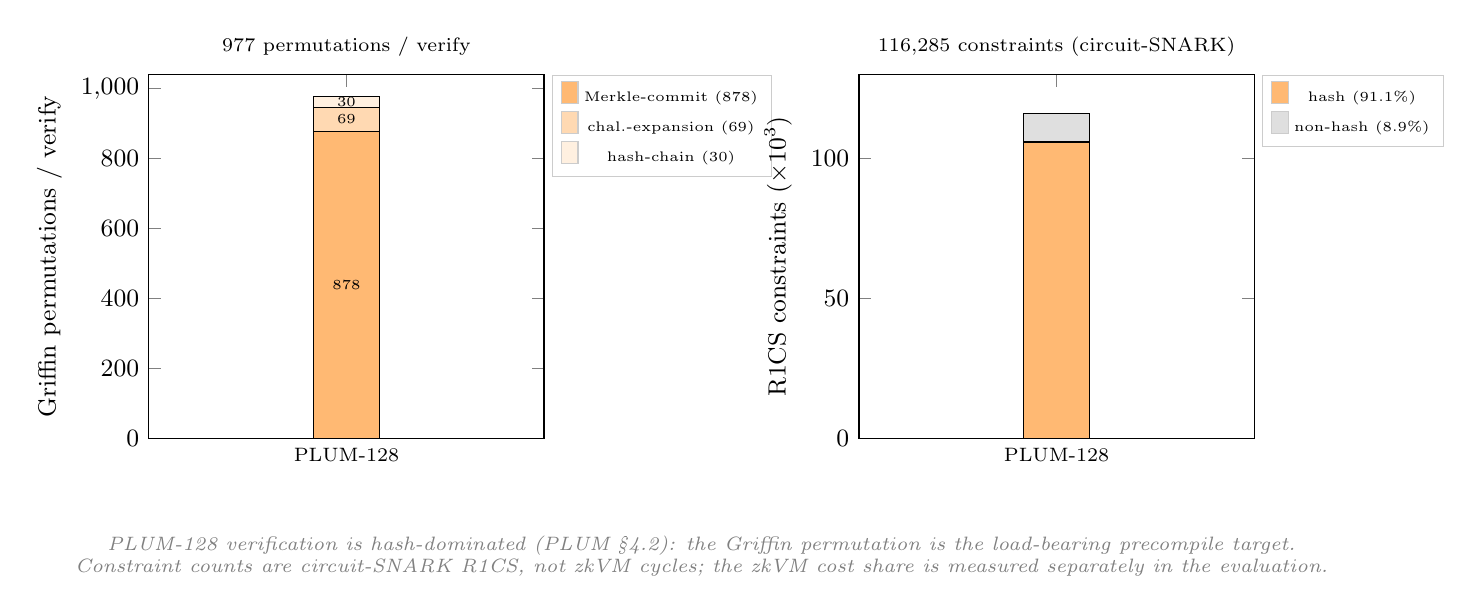
\begin{tikzpicture}
% ---- left: the 977 Griffin permutations broken down ----
\begin{axis}[
  name=perms,
  width=6.6cm, height=6.2cm,
  ybar stacked, bar width=24pt,
  ymin=0, ymax=1040,
  ylabel={Griffin permutations / verify},
  symbolic x coords={PLUM-128}, xtick=data, xticklabel style={font=\scriptsize},
  title={\scriptsize 977 permutations / verify}, title style={yshift=-1mm},
  legend style={at={(1.02,1)},anchor=north west,font=\tiny,draw=gray!40},
  every node near coord/.append style={font=\tiny}, nodes near coords,
  font=\small,
]
\addplot[fill=orange!55] coordinates {(PLUM-128,878)}; \addlegendentry{Merkle-commit (878)}
\addplot[fill=orange!30] coordinates {(PLUM-128,69)};  \addlegendentry{chal.-expansion (69)}
\addplot[fill=orange!12] coordinates {(PLUM-128,30)};  \addlegendentry{hash-chain (30)}
\end{axis}
% ---- right: the 91.1% R1CS constraint share (shifted well clear of left legend) ----
\begin{axis}[
  name=share, at={($(perms.east)+(4.0cm,0)$)}, anchor=west,
  width=6.6cm, height=6.2cm,
  ybar stacked, bar width=24pt,
  ymin=0, ymax=130,
  ylabel={R1CS constraints ($\times 10^{3}$)},
  symbolic x coords={PLUM-128}, xtick=data, xticklabel style={font=\scriptsize},
  title={\scriptsize 116{,}285 constraints (circuit-SNARK)}, title style={yshift=-1mm},
  legend style={at={(1.02,1)},anchor=north west,font=\tiny,draw=gray!40},
  font=\small,
]
\addplot[fill=orange!55] coordinates {(PLUM-128,105.952)}; \addlegendentry{hash (91.1\%)}
\addplot[fill=gray!25]   coordinates {(PLUM-128,10.333)};  \addlegendentry{non-hash (8.9\%)}
\end{axis}
% caption placed well below both axes, full width
\node[font=\scriptsize\itshape,gray,align=center,anchor=north]
  at ($(perms.below south west)!0.5!(share.below south east)+(0,-0.7cm)$)
  {PLUM-128 verification is hash-dominated (PLUM \S4.2): the Griffin permutation is the
   load-bearing precompile target.\\
   Constraint counts are circuit-SNARK R1CS, not zkVM cycles; the zkVM cost share is
   measured separately in the evaluation.};
\end{tikzpicture}
\end{document}
